\newtheorem{proposition}{Proposition}
\newtheorem{remark}{Remark}
\newtheorem{lemma}{Lemma}
\newtheorem{corollary}{Corollary}
\newtheorem{example}{Example}

\documentclass[11pt]{article}

\usepackage{amssymb}
\usepackage{graphics}
\usepackage{amsmath}
\usepackage{verbatim}
\usepackage{setspace}
\usepackage{color}
\usepackage{ulem}
\usepackage{sectsty}
\usepackage{hyperref}
\sectionfont{\large}
\usepackage{graphicx}
\def\bs{\boldsymbol}


\usepackage{xr}
\externaldocument{covidEffectOfNPI-revision}

%\renewcommand{\sout}[1]{}
%\renewcommand{\bf}{}

\newtheorem{assumption}{Assumption}
\setlength{\topmargin}{-1cm}
\setlength{\oddsidemargin}{0.25cm}
\setlength{\evensidemargin}{-0.2cm} \setlength{\textheight}{22cm}
\setlength{\textwidth}{16cm}
\onehalfspacing
\def\thebibliography#1{\section*{References\markboth
  {REFERENCES}{REFERENCES}}\list
  {}{\settowidth\labelwidth{}\leftmargin\labelwidth
  \advance\leftmargin\labelsep
  \usecounter{enumi}}
  \def\newblock{\hskip .11em plus .33em minus -.07em}
  \sloppy
  \sfcode`\.=1000\relax}
  
  \pdfminorversion=4

\begin{document}


\newcommand{\replytitle}
{
\subsection*{Reply to the Comments on  ``Causal Impact of Masks, Policies, Behavior on Early COVID-19 Pandemic in The U.S.''}
}

\newcommand{\refreplyheading}
{Thank you very much for your helpful and constructive comments on our paper. We appreciate the time you spent in reviewing this paper. We have followed your recommendations, and those of the other reviewers', as far as possible.
Major changes are:}
 

\newcommand{\changes}
{
\begin{enumerate}

\item   We  state the limitations of our work with cautious notes on interpreting our causal model.
\item   Following the editor's suggestion, Section 2 is reorganized and we improve our discussion on the testable restrictions. Tables 7 and 9 in Section 3 provide   an  over-identification test for no indirect effect of mask policy on case/death growth via behavior.
\item   Following suggestions by the editor and the referees, we provide various sensitivity checks as well as the results of debiased fixed effects estimator  in Section 4.

\item Given Referee 1's comment, all regressions now include a dummy for state governor's party and its interaction with month dummies as additional controls.

\item   We improve the figures for counterfactual experiments so that they are now easier to understand. 

\item We now combine movie theater closures, restaurant closures, and non-essential business closures as one policy variable called ``business closure policies'' by taking the average of these three variables. Accordingly, we conduct a counterfactual of keeping all business open. 

\item We changed the starting date of mask mandates to March 14th in our counterfactual experiment of mandatory mask policy.

\item  We adjusted the timing of monthly dummies for estimating behavior equation ($PI \to B$)  in Table 3.  In the previous version, the definition of monthly dummies for behavior equation ($PI \to B$) is different from that for case growth equation ($BPI \to Y$)  or ($PI \to Y$). This issue is now fixed.
%\item We made some grammatical adjustments.
\end{enumerate}

%No other changes of substance are made.
}

\replytitle
\subsection*{Reply to Editor}
\refreplyheading
 
\changes


In addition to our reply to the referee report, we also attached our reply to the comments we have received from
C. Jessica E. Metcalf (\url{https://metcalflab.princeton.edu/people/metcalf-c-jessica/}) who gave us a set of detailed comments via private communication.





\subsection*{Reply to Editor's Comments}
\begin{itemize}

\item   \textit{``I particularly like your mapping of your estimating equation to the SIR model. But, it would be nice to discuss further the assumptions in light of the SIR model. For example, how do the orthogonality assumptions in (1) relate to the assumptions on top of page (14)? and just to be clear, you have a "causal model" yet for identification you rely on projections in the random effects specification (and no exclusion restriction). For example, what do you rule out vis a vis "diff in diff" type event study models with fixed effects? How about a brief discussion of the "invariance assumption" and why you think it would hold in your counterfactual exercise. ''}

Thank you. The testable restrictions of the model are now described better.  Please see the discussion around equation (TR). The SIR model
for example implies that testing rate is a confounder for case growth rate, but the causal model implies  that testing rate
does not affect the behavior or policy variables (other than through cases). This is an overidentification restriction.
To show the power of this approach, we also looked at imposition of other "contextual information": for example, mask
having only direct effect on growth rates (and not via behavior) or business closure policies affecting case growth rates
only through behavhior.

The fixed effect estimates lump state-level confounders in one unobservable component.  Our approach does not preclude
the use of fixed effects to estimate the model. We present fixed effects as part of Sensitivity analysis.

The invariance assumption is similar to standard assumptions in Structural VAR literature, starting with Sims (1972).
 

\item   \textit{``It might make sense to reorganize Section 2 (which is the heart of the theory in the paper) into a simpler to read section  where the assumptions that are required for causal interpretation are laid out. Also, one easier threshold is that your system of estimating equations provide a direct "predictive effect" of various policies. These predictive (not causal) in my opinion would still be very useful. ''}

Following your suggestion, we have reorganized Section 2. 
 We also state the following in abstract:
 \begin{quote}
 We stress that our study is observational and therefore should be interpreted with great caution. 
 From a completely agnostic point of view,
our findings uncover predictive effects (association) of observed policies and behavioral changes  on future health outcomes,
 controlling for informational and other confounding variables.
\end{quote}

\end{itemize}


\newpage

\replytitle
\subsection*{Reply to Referee 1}
\refreplyheading

\changes
\subsection*{Reply to Referee 1's Comments}
\begin{itemize}

\item  \textit{``I think it would be helpful if the authors clearly state the limitations of their work and
cautiously warn that their casual impact cannot be interpreted too literally.''}
 
 This point is valid.  We added a cautionary message to the abstract. Furthermore,
 we added the following paragraph to Section 2.2. 
 \begin{quote}
 Validation of the model by (TR) allows us to check exclusion restrictions brought by contextual knowledge, and check stability of the model by using different data subsets. However, passing the (TR) does not, of course, guarantee that the model is necessarily valid for recovery of causal effects. The only fundamental way to truly validate a causal model for observational data is through a controlled experiment, which is impossible to carry in our setting. We shall however cross-check our results against other scientific evidence and, for example, results from RCT on effectiveness of masks on respiratory deceases (though not in the Covid-19 context).
 \end{quote}
 
 We also state the following in abstract:
 \begin{quote}
 From a completely agnostic point of view,
our findings uncover predictive effects (association) of observed policies and behavioral changes  on future health outcomes,
 controlling for informational and other confounding variables.
\end{quote}
  
\item[1.]   \textit{(Source of state-level variation) ``The main specification is based on random effects panel data
models. It is unclear what is the source of state-level variation. In particular, what is behind
the difference in mask policies across the states? Is this mainly driven by political partisanship?
To argue that the current paper credibly identifies the casual impact of masks for
employees, could the economics profession be persuaded that adopting masks for employees
is sufficiently random conditional on observed confounders? The paper provides some
discussions; however, more thorough discussions would be highly valuable.''}
  
We provide various sensitivity checks: First, we now include governor's party affiliation as an additional state-level variable in random effects specification. 
Second, we exclude the state of New York from the sample because it may be viewed as an
outlier in the early pandemic period and it is  one of the states that adopted mandatory mask policies in April. Third, we added mask wearing rates in Mach and April from survey as an additional regressor to control for unobserved personal risk-aversion and people's initial attitude for mask wearing. Fourth,  we added the log of Trump's vote share in 2016 presidential election as confounder for
unobserved private behavioral response. Fifth, we report the fixed effects estimator that controls for latent state confounders as components of $W_{it}$.  
As shown in the paper, the estimated coefficient of masks for employees is not so sensitive with respect to excluding NY as well as adding more controls that are possibly important confounders.  The results of other policies are less robust/uncertain and we clearly communicate this in the abstract and in the introduction.

As stated below, we also examine a specification that includes lagged behavior variables as information; employed the Double Machine Learning (DML) with Lasso for dimensionality reduction of confounders as well as the DML with Random Forest for dimensionality reduction and capturing potential nonlinearity of confounders. We find that the estimated coefficients of masks for employees are robust with respect to alternative specifications and methods. Other coefficients on other policies are less robust
(but helpful effects of these policies can not be ruled out).
  
  
\item[2. ]  \textit{(Information structure) ``I think it is really nice that the paper emphasizes the importance of
information structure. Having said this, section 2.2 is quite limited because the most extensive
form of information structure consists of time effects and lagged and integrated effects
of state-level cases and deaths. I am puzzled what sense these form information structure. It
is unclear to me why lagged values of policies and behavior are not part of the information 
structure. I think it would be useful to provide remarks regarding the limitation of the current
information structure and acknowledge that the estimation results and in particular the
simulated counterfactuals are crucially dependent on it.''}
  
We chose information structure that is parsimonious and yet, we believe, captures the  information that is most relevant for people's behavior (at the minimum, it captures our own behaviors). This information structure is also in line with CDC guidelines
for policies, which
is formulated in terms of observed infection of outcomes and not in terms of behavior.

Conditioning on current policy variables that is included in all specifications, the lagged values of policies will  likely add little additional information and, therefore, we decided to exclude lagged values of policies from the information structure. We are 
completely free to interpret that the coefficient of current policy variables has both informational content and behavior-constraining effect.

On the other hand, the lagged values of  behaviors may be a part of the information structure. As a sensitivity check, we estimated a specification that includes  lagged behavior variables as information variables in Section 5. The mask policies 
appear to be robust withe respect to the inclusion of these variables. The effects of business closures appear to be less
robust -- the estimated effects become more attenuated, and we report these findings in the conclusion. 
  
\item[3.]  \textit{(Expectation and Lucas critique) ``Related to the previous comment, what would be the link
between the current paper's setup and how expectations are formed given the information
structure? For example, is this paper safe from Lucas critique? Some comments would be
helpful.''}

In our view, people's mobility decisions are largely based on the current information and people's expectation of future cases/deaths is not the first order importance when people make their mobility decisions because there is no obvious inter-temporal substitution with respect to their mobility decisions. 
    
Also, given a lack of expectation data, statistically testing whether expectation over future cases/deaths is important as a determinant of people's behavior is difficult in this context. For example, including future realized cases/deaths as an additional regressor in the behavior equation leads to the positive estimate because of the reverse causality, i.e., an increase in mobility leads to an increase in future cases.
  
\item[4.]  \textit{(Causal ordering) ``It is assumed in the paper (on page 8) that behavior is affected by policies
but not the other way. This is certainly an important exclusion restriction that the paper
depends on. This may be a reasonable first-order approximation, but it could be that some
polices are formed by behavior (such as online petition and so on). It would be useful if
the authors could add some more remarks why the causal chain on pages 8-10 is plausible
and acknowledge that the results in the paper are highly conditional on this particular causal
ordering.''}

Thank you for your comment. Following your comment, we added the following sentence:
\begin{quote}
The  lagged values of behavior variable may be also included in the information set, but we postpone this discussion after the main empirical results are presented.
\end{quote} 
As a part of sensitivity checks, we now examine if the estimates are sensitive when we include two weeks lagged value of behavior variables in the information set, under which policies depend on past behavior. We find that the estimated coefficients of masks for employees are not sensitive to an inclusion of past behavior variables. 
 
We think it is reasonable to assume that people's behavior today will not immediately affect today's policy because it takes time for policy makers to gather information on people's behavior and make a policy decision based on gathered information, especially in the early pandemic period.   Moreover, CDC guidelines don't seem to rely on people's behavior but on measured infection outcomes.
  
\item[5.]  \textit{(Details about confidence intervals) ``Starting from Figure 1, confidence intervals are shown
in the shaded region. It is not clearly stated in the paper how they are obtained. On page 32,
in Figure 9, the authors state:
We set initial $\Delta\log\Delta C$ and $\log\Delta C$  to their values first observed in the state we
are simulating. We hold all other regressors at their observed values. Error terms
are drawn with replacement from the residuals. We do this many times and report
the average over draws of the residuals. The shaded region is a point-wise 90\%
confidence interval. It is still unclear how a pointwise confidence interval is obtained. Does this mean that a pointwise
90\% confidence interval is constructed by simulation or bootstrap? It would be useful if the authors describe how to construct a confidence interval and provide a remark why it is valid.''}

Thank you! We have added a much more detailed discussion and also an appendix where the details
are explained.
  
\item[6.]  \textit{(Replication files) ``It would be great if the authors could post their dataset and replication
files on public domain such as a GitHub page or ICPSR at https://www.openicpsr.org/
openicpsr/covid19.''}

All programs and dataset will be available at our GitHub page, which is currently set to be private but we will plan to make it publicly accessible once the final version of the paper is accepted.
  
\item[7.]  \textit{(Debiased fixed effect estimates) ``On page 11, the authors state:
However, we find the debiased fixed effect estimates are qualitatively and quantitatively
similar to the correlated random effects estimates. Given this finding,
we chose to focus on the latter, as it is a more standard and familiar method, and
report the former estimates in the supplementary materials for this paper.
Could the authors kindly point out where the supplementary materials are? Perhaps I did not
locate them properly, but the appendices do not seem to include the results from debiased
fixed effect estimates.''}

We now present the results of the debiased fixed effect estimates in Table 8 in Section 4.2. 
  
\item[8.]  \textit{(Random effects vs. fixed effects) ``In addition to the previous comment, another reason for
preferring the random effects model could be that there could be substantial measurement
errors in behavior and policy variables. Fixed effects estimators could suffer more from measurement
errors.''}

Following your suggestion, we have added the following paragraph:
\begin{quote}
The results in Table \ref{tab:PtoY-fe} should be interpreted with caution. The fixed effects approach may not be preferred to random effects approach here because the former relies on long time and cross-sectional histories but, in our data, the effective time-dimension is short and a number of states is not large. Furthermore, the fixed effects approach could suffer more from  measurement errors, which could be a concern for our behavior and policy variables.
\end{quote}
  
\item[9.]  \textit{(Multiple testing) ``There are lots of hypotheses and stars in Tables 3-7. Perhaps it might be
useful to consider multiple testing corrections by controlling the familywise error rate or a
related concept.''}

We are not doing any hypothesis testing in this paper: we are constructing point and interval predictions for 2-3 key policies. This
is in line with with IHME institute is doing (our analysis on masks predates theirs, as we posted our findings
at the end of May, and they announced their findings in middle of July). The 
"asteriks" are reported as a matter of statistical convention, but we never use them in any formal way. We could probably
erase them and proceed in asterikless fashion.

Furthermore, we believe that testing "no mask effect" hypothesis is actually not an interesting exercise for policy analysis
or actual policy decisions.   From a decision-theoretic point of view the cost of accepting the false null is extremely high,
which could result in huge losses. The Neyman-Pearson test with level $\alpha=$ small, corresponds to the idea that the cost
of falsely rejecting the null is small (little harm done if the "no mask effect" is falsely accepted), e.g. Amemiya "Introduction to Statistics and Econometrics".  So doing "no mask effect" testing with very low $\alpha$ would correspond to assuming that the cost of deciding that masks are not effective is very low.  The potential cost of accepting the null, if it is false, is just huge.   Multiple hypothesis testing would further drive $\alpha$ to smaller values, and we are not sure how this would align with the decision-theoretic framework.

%Remark. Elaborating further on decision-theoretic point, with $H_0$ masks being useless, the policy makers problem is to make a decision 
%to achieve minimal loss:
%$$
%\min (E [Loss (NoMask) | H_0] P[H_0], E [Loss (Mask) | H_A] P[H_A]).
%$$
%The optimal decision is not to use Masks if $$P[H_0]> \alpha = P[H_A] \cdot E [Loss (Mask) | H_A] /E [Loss (NoMask) | H_0] ),$$
%which gives the relevant $\alpha$. E.g, using $\alpha =.1$ results from the information that $P[H_A]=1/2$ and assuming that the loss from using masks has to be 5 times higher than the loss from not using masks. 


 For masks, given the decision-theoretic framework, given prior evidence from RCT on efficacy of masks for respiratory deceases, (unfortunately not including corona), the interesting nulls would be "mask effects  have -.15, -.1, -.05" effects on growth rate. This null would not be  rejected no matter what adjustments to p-values we make or what sensitivity analysis we make.  Moreover, after doing all of the sensitivity exercises, we would not be able to reject this null.   This corresponds to the idea that the null hypothesis
 here is the one that is very costly if falsely rejected.



  
\item[10.]  \textit{(Table 3A: Cases as Information) ``It is puzzling why the coefficients on  $\Delta\log\Delta C$ are positive
and large. How would the authors interpret these numbers? Would this mean that information
on lagged growth rates in new cases encourages people to become more mobile?
Probably I am mistaken. It would be helpful if the authors could clarify this.''}

In columns (1)-(4) of Table 3(A), the estimated coefficients on $\log\Delta C_{it}$ is negative and the sum of estimated coefficients of $\Delta \log\Delta C_{it} $ and $\log\Delta C_{it}$ are also negative except for grocery.

To interpret these results, rewrite a regression specification after omitting other variables as 
$B_{it} =  \gamma_1 \Delta \log\Delta C_{it} + \gamma_2   \log\Delta C_{it} =  (\gamma_1 +\gamma_2) \log\Delta C_{it} - \gamma_1   \log\Delta C_{i,t-7}$.
In columns (1)-(4) of Table 3(A),  the estimated values of both $(\gamma_1 +\gamma_2)$ and $-\gamma_1$ are negative except for grocery. This suggests that  a higher \textit{level} of confirmed cases reduces people's mobility in workplaces, retails, and transit. For grocery, the positive estimated coefficient of $(\gamma_1 +\gamma_2)$ may reflect stock-piling behavior in early pandemic periods.
  
 We also note that the estimated coefficients of  $\Delta \log\Delta D_{it} $ and $\log\Delta D_{it}$ are negative in columns (1)-(4) of  Table 3(B), consistent with a hypothesis that a higher number of deaths as well as a higher growth rate of deaths reduces people's mobility.
 
Following your suggestion, we added the above discussion in footnote X (check!) when we discuss in Table 3A.


\item[11.]  \textit{Figure 8 is very informative. Perhaps the authors could show this in introduction as well.''}

We thought about this suggestion but, eventually, we can keep it as it is.
  
  \end{itemize}
  
  
\subsection*{Reply to Referee 1's Minor Comments}
\begin{itemize}


\item[1.]  \textit{(Figure 1) ``What are black and grey dotted lines? It would be helpful if the authors add notes
to the figure. The same questions apply to Figures 2 and 3 and other figures.''}

Black and grey dots represent each state's change in growth rate over time.  Given that it may be difficult to digest a counterfactual change in case/death growth in introduction, we decided to focus on relative effect of policies in Figures 1-3. 

\item[2.]  \textit{(Figure 4) ``What do S. \& P. stand for in Figure 4?''}

It stands for 
P. Wright and S. Wright as discussed in the footnote 2:
\begin{quote}
The father and son,
P. Wright and S. Wright closely collaborated to develop structural equation models and causal path diagrams; P. Wright's
key work represented supply-demand system as a directed acyclical graph and established its identification using
exclusion restrictions on instrumental variables.
\end{quote}

\item[3.]  \textit{(Footnote 17) ``Is this necessary? This seems obvious. The authors could simply drop this
footnote or make it more informative.''}

Following your suggestion, we have dropped this footnote. 

\item[4.]  \textit{(Footnote 19) ``On page 17, in footnote 19, the authors state:
We drop ``Residential' because it is highly correlated with both ``Workplace'' and
``Retail \& recreation" at correlation coefficients of 0.98.
This sentence is ambiguous. Do the authors mean that both correlation coefficients are identically 0.98? Please rephrase this sentence.''}

We rephrased this sentence as follows: `` We drop ``Residential'' because it is highly correlated with  ``Workplaces'' and  ``Retail \& recreation''  at correlation coefficients of -0.98 and -0.97, respectively. ''

\item[5.]  \textit{(Figures 9 and 11) ``On page 32, in Figure 9, the subfigures in the middle and right panels
contain non-legible legend. Please improve the figures. The same applies to Figure 11 and
other similar figures in the appendix.''}

We have decided to drop these legends to improve the readability of those figures. 

\item[6. ]  \textit{(Intepretation) ``On page 13, it is state that
The estimates imply that mandating masks on April 1st would have led to 500
fewer cases and 250 fewer deaths in Washington by the start of June.
What is the time scale of this statement? Does this mean 500 fewer cases weekly or in total
by the start of June? Please clarify the quantitative statement.''}

It is in total by the start of June. We have modified the sentence as suggested.  

\item[7.]  \textit{``Some of the figures are difficult to read because there are too many curves. In particular,
Figures 18, 19, and 21 convey very little information. Please improve the figures and delete
some of them if they are less important.''}

Following your suggestion, we have consolidated these figures and present figures with quantiles to improve the readability.

\end{itemize} 
 
\newpage

\replytitle
\subsection*{Reply to Comments by C. Jessica E. Metcalf }
\refreplyheading

\changes
\subsection*{Reply to Comments  by C. Jessica E. Metcalf }
\begin{enumerate}

\item  \textit{``My sense is that the delay between infection and case reporting should be closer to a week (more in specific comments below) and various lines of evidence suggest two waves of death following infection, one early and one late (e.g., in https://science.sciencemag.org/content/369/6500/208: "We identify two clear subpopulations among hospitalized cases: individuals that die quickly after hospital admission (15\% of fatal cases, with a mean time to death of 0.67 days) and individuals who die after longer time periods (85\% of fatal cases, with a mean time to death of 13.2 days) (fig. S3)."). Presumably the preoponderance of weight at the later time should minimize the effects on your estimates... I think a sensitivity analysis to this would be desirable - as well as a reference to some of the literature beyond that written by economists... My sense is that the number is closer to 6 days or a week? But I have not reviewed that literature recently (Table 2 in this seems to suggest that aligns... https://www.cdc.gov/coronavirus/2019-ncov/hcp/planning-scenarios.html)"}

Following your suggestion,   we provide a sensitivity analysis on the delay between infection and case reporting (or death reporting) in Section 4.2. The timing was motivated by a careful reading of Table 2 referenced above.

\item \textit{``the collinearities, and lack of agreement in cases/deaths makes the separate estimates for different policies really rather uncertain? We would all love a crisp statement about the effects of masks.... but I wonder if Figure 1 gives a sufficiently robust sense of the uncertainty  based on the estimates provided?''}
 
Given  your suggestion, Figure 9 presents whisker-dot-plots for confidence intervals of mask coefficients (as well as other policy variables) across different specifications, timing assumptions, and estimation methods. We believe these figures provide a sufficient robust sense of the uncertainty on the  estimates. 
  
\item \textit{`` Figure 1 - are the points on the left hand figures the state specific estimates? or? What is the blue enveloppe? Mildly distracting having nothing happen till halfway through April (I know this is purely illustration, but an 'all else equal' in the caption might help?) And then, for what happens next, crudely, log(It/It-1) is diminshed by a factor by masks, etc, and the lag is simply due to the delays until cases? ''}
 
Black and grey dots represent each state's change in growth rate over time.  Given that it may be difficult to digest a counterfactual change in case/death growth in introduction, we decided to focus on relative effect of policies in Figures 1-3.
  
We changed the starting date for counterfactual figures.

\item \textit{`` p5 - perhaps some papers from beyond the Econ literature would be relevant for a sense of the status of our knowledge of the epidemiogogy?  ''}

We have reviewed and added more references from the epidemiology literature. See, for example, footnote 9.
There are also many more references in the Into other than Econ literature.

\item \textit{`` p6 - simulations would produce exponential spread of disease - well, yes? The mechanism is reasonably well described, and the conditions to elude exponential growth are fairly crisp - even if you include 'a voluntary behavioral response' the outcome will be exponential growth unless you are in a regime where susceptible depletion is dominating dynamics, or you have shifted Re$<$1.  ''}
 
 Thank you for raising this issue. Yes, you are right. Following your comment, we have changed the sentence as follows:
\begin{quote}
When such a voluntary behavioral response is ignored, simulations would necessarily exhibit exponential spread and over-predict  cases and deaths. In contrast, as cases and deaths rise, a voluntary behavioral response may possibly reduce the effective reproduction number  below 1,  potentially preventing exponential spread. Our counterfactual experiments  illustrate the importance of this voluntary behavioral change. 
\end{quote}
 

\item \textit{`` p20 log delta C\_it is obviously strongly autocorrelated (on top of the other collinearities detailed) - I also wondered if time since start of the outbreak might not do just as well at capturing the dirve in change in behavior? Do numbers of cases and deaths do better? ''}

The autocorrelation component is captured by the lags of this variable in the dynamic specification. In addition,
we cluster the standard errors by state (capturing the impact of temporal dependence in the series, 
not accounted for by the lag structure).

We believe that it is better to use the number of cases and deaths rather than time since start of the outbreak as a  general framework to analyze the spread of COVID-19. This is especially true if we analyze the second wave of COVID-19, where time since start of the first outbreak may not be so relevant, and identifying the start of the second outbreak may be difficult. 



\item \textit{`` Figure 8 - I do like seeing the data, but it also just raises questions, as you say, confounders + many other things at play.... I wondered if there would be a way to create a visual that captured a bit more of this, and pinpointed the anomalies which are where the inferential power lies. ''}

This is an interesting suggestion. We thought about the possibility of providing a version of Figure 8 (now, Figure 10) based on the regression residuals after taking out the effect of confounders etc but, eventually, we decided not to present such results due to the space constraint.  


For your reference, we have constructed a version of  figure based on the residuals of regressing the case or death growth rates on state characteristics, month dummies, and their interactions, which illustrates that states with a mask mandate tend to have lower case and death growths even after controlling for confounders.    % and then computing their average value for states with or without a mask mandate for each date. 

\begin{figure}[ht]
  \caption{Average  residuals of regressing case and death growth on confounders among states with or without  mask mandates \label{fig:masks-res}}\vspace{0.2cm}
 \begin{minipage}{\linewidth}
    \centering
    \begin{tabular}{cc}
      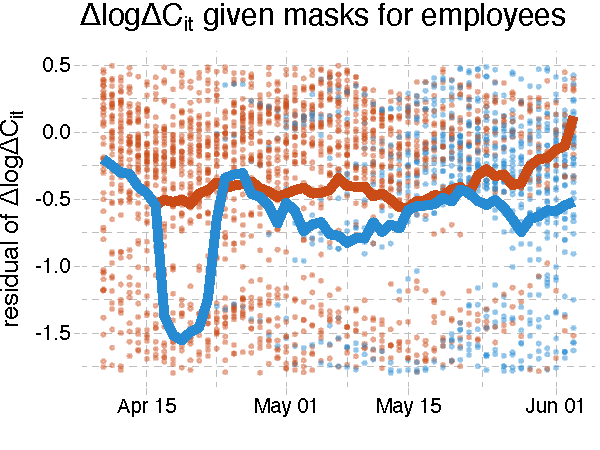
\includegraphics[width=0.5\textwidth]{tables_and_figures/pmaskbus-cases-res-14}
      &
        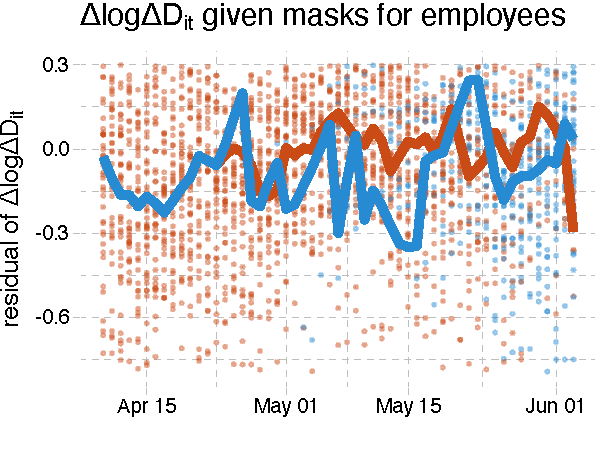
\includegraphics[width=0.5\textwidth]{tables_and_figures/pmaskbus-deaths-res-21}
    \end{tabular}
    \begin{flushleft}
      \scriptsize In these figures, red points are the regression residuals of case or death
      growth rate on confounders in states without a mask mandate. Blue points are
      states with a mask mandate 14 (21 for deaths) days prior. The
      red line is the average across states without a mask mandate 14
      (21 for deaths) days earlier. The blue line is the average
      across states with a mask mandate 14 (21 for deaths) earlier.
    \end{flushleft}
  \end{minipage}
\end{figure}



\end{enumerate}


\end{document}